\section{Analysis}
\label{sec:Analysis}

As a first step, the invariant mass of the simulated $B_s \to \psi(2S)K_S$ decay is visualized in \autoref{fig:sim_mass}.
\begin{figure}[H]
	\centering
	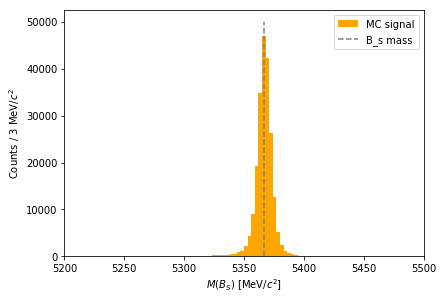
\includegraphics[width=0.5\linewidth]{plots/simulation_mass.png}
	\caption{Reconstructed invariant mass of the simulated $B_s \to \psi(2S)K_S$ decay.}
	\label{fig:sim_mass}
\end{figure}
A sharp peak is visible around the nominal $B_s$ mass, which is expect as the Monte Carlo simulation of this decay only simulates a signal without any background.
Using this distribution, a signal window is defined as the smallest possible intervall containing \qty{99}{\percent} of the events in the simulation sample.
The resulting signal intervall is
\begin{equation*}
    I_\text{sig} = [5333.4, \, 5394.6] \, \si{\mega\electronvolt\per c^2}.
\end{equation*}
The reconstructed mass of real data collected at the LHCb experiment is shown in \autoref{fig:data_mass}.
\begin{figure}[H]
	\centering
	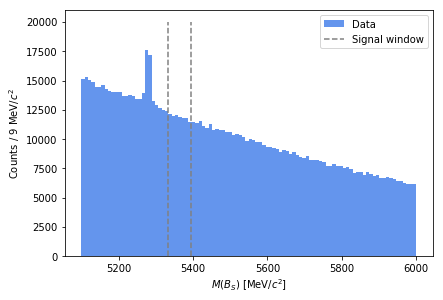
\includegraphics[width=0.5\linewidth]{plots/signal_window.png}
	\caption{Reconstructed invariant mass of $B^0$ candidates from LHCb data.}
	\label{fig:data_mass}
\end{figure}
As the data has already been preselected, a peak around the nominal $B^0$ mass is directly visible without any further selection. However, the $B_s$ peak inside the signal window
is still hidden due to the large amount of combinatorial background remaining in the data.

\subsection{Feature selection}
In order to train a multivariate classifier, suitable features have to be selected that can provide unbiased and meaningful information to the classifier.
The first important aspect is that the features have to be well simulated, meaning they have to show good agreement with actual data. To obtain a data sample consiting of only signal
events like the simulation, so called s-weights have already been computed for the data. Applying these s-weights to the data will lead to only signal-like events remaing, as 
it can be seen in \autoref{fig:sweights}.
\begin{figure}[H]
	\centering
	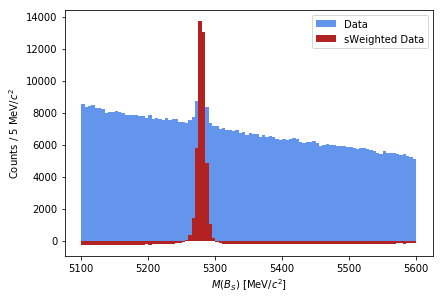
\includegraphics[width=0.5\linewidth]{plots/sweights.png}
	\caption{Data with and without applied s-weights.}
	\label{fig:sweights}
\end{figure}
Now, the distributions of the sweighted data and control simulation can be compared. The control simulation is used here because the sweights were determined in respect to the
$B^0$ decay, as this is alot more prominant in the data. Additionally, kinematic weights are applied to the control simulation which further improve the accuracy of the distributions.
A weighted Kolmogorov Smirnov test is performed using \eqref{eq:ks_test}, the resulting test statisitc is a measure for how similar the distributions are. 
Subsequently, all features with a test statistic $< \, 0.1$ are removed. 
The same procedure is performed again with the data and signal simulation, however now the remaining feautures are checked for their discriminating power.
This is archieved by using the upper mass sideband of the data (reconstructed mass above signal window), as these candidates only contain combinatorial background. Consequently,
only feautures with with a test statisitc $> \, 0.5$ are kept, which ensures that the classifier gets features from which it can learn clear differences from signal and background.
The remaining feautures are checked for their correlation in respect to the invariant $B^0$ mass, all attributes with a correlation above $0.1$ are discarded, as these
could introduce a bias in the classifier. Lastly, the correlation of the leftover features is computed in respect to each other. Highly correlated attributes are removed as they
only provide redundant information. In total, 16 features remain after all requirements.
A few examples of the disitributions of selected features are shown in \autoref{fig:BDT_vars}.
\begin{figure}[H]
	\centering
	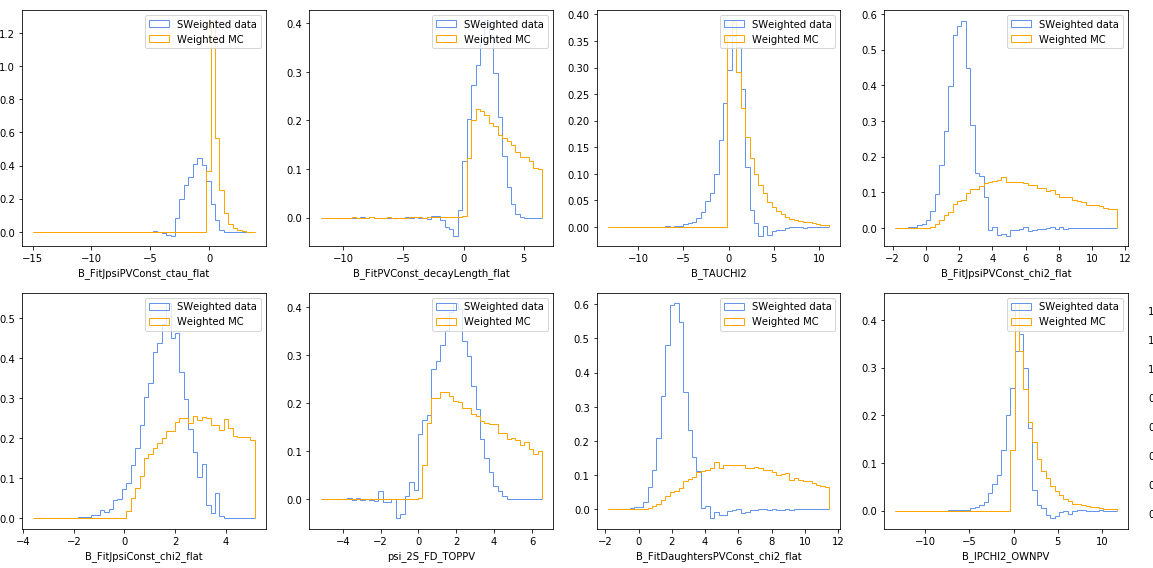
\includegraphics[width=0.8\linewidth]{plots/BDT_variables.png}
	\caption{Some examples for the distributions of features selected for the classifier training.}
	\label{fig:BDT_vars}
\end{figure}
These distributions show clear differences between signal and background, while also ensuring they are correctly modeled. This ensures that the classifier will learn the
differences between signal and background and not between data and simulation.

\subsection{Classifier training}
As explained in the beginning, the classifier used in this analysis is a gradient boosted decision tree. Its implemantation is done using the \texttt{XGBoost} package \cite{XGBoost}.
The signal proxy are all events of the signal simulation inside the previously determined signal window. As a background proxy, all events in the data sample with an invariant mass
larger than the signal window are selected. Again, kinematic weights are applied to the signal simulation. The background events are also assigned with a weight that ensures that the
classifier sees an equal amount of signal and background events.
A five-fold cross validation is used during the training, resulting in five individual BDTs. Their performace is nearly identical, verifying this is important to avoid overtraining.
The results and scores of the first BDT are shown in the following \autoref{fig:BDT_1}.
\begin{figure}[H]
	\centering
	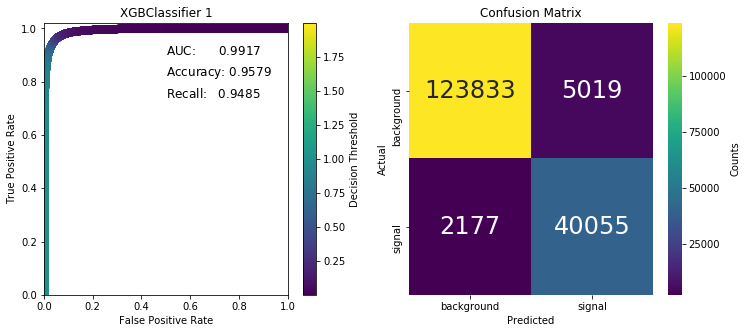
\includegraphics[width=0.8\linewidth]{plots/BDT_1.png}
	\caption{Results and scores of the first BDT.}
	\label{fig:BDT_1}
\end{figure}
The area under the ROC curve as well as precision and recall are all high, indicating a succesfull training.
The response of this BDT for training and test data can be seen in \autoref{fig:BDT_1_pred}.
\begin{figure}[H]
	\centering
	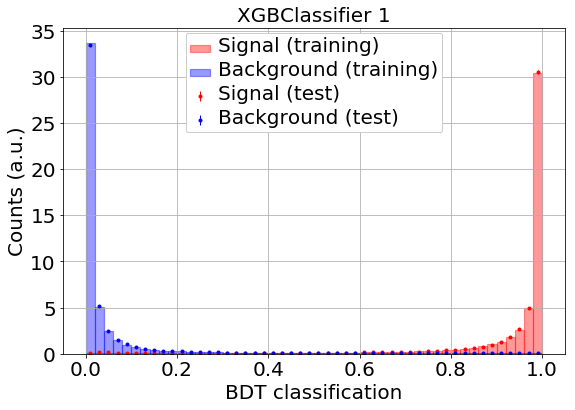
\includegraphics[width=0.5\linewidth]{plots/BDT1_pred.png}
	\caption{Response of the first BDT to training and testing data.}
	\label{fig:BDT_1_pred}
\end{figure}
A very similar response to training and test data is oberved, further verifying that no overtraining has occured.
The remaining results of the other four BDTs can be found in the appendix.

\subsection{Threshold optimization}

To obtain the optimal cut on the prediction of the five BDTs, the Punzi Figure of Merit (POM) is used \eqref{eq:fom}.
For varying threshold values, the signal efficiency and number of background events in the signal window is computed after the respective BDT cut.
The signal efficiency simply describes the ratio of signal events before and after the BDT cut. In contrast, the number of background events in the signal
window is computed by fitting an exponential background model to the upper sideband and extrapolating the number of events in the desired signal region.
This is done seperately for each BDT, the resulting five FOMs are plotted in \autoref{fig:FOM}.
\begin{figure}[H]
	\centering
	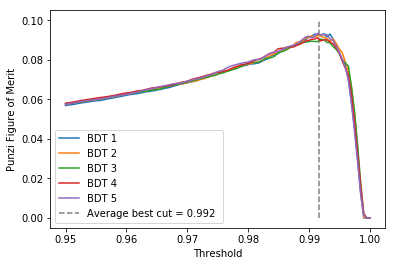
\includegraphics[width=0.6\linewidth]{plots/FOM.png}
	\caption{FOM for the five individual BDT including the averaged best cut.}
	\label{fig:FOM}
\end{figure}
The optimal cut is now determined as the average of the maxima of the five FOMs and also shown in \autoref{fig:FOM}.

\subsection{Determination of the signal yield}

As the best cut has now been determined, the BDT can predict on the data and a corresponding cut is made on the BDT prediction. The following \autoref{fig:data_BDT} shows the
data after this procedure.
\begin{figure}[H]
	\centering
	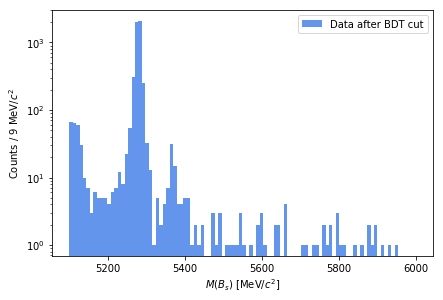
\includegraphics[width=0.5\linewidth]{plots/data_BDT.png}
	\caption{Distribution of the invariant $B^0$ mass in data after the BDT has been applied.}
	\label{fig:data_BDT}
\end{figure}
While the $B^0$ peak is still clearly visible as before, the second $B_s$ peak can now also be seen.
To calculate the yield of $B_s$ decays, a fit has to be performed on the data.
A large amount of partially reconstructed events is visible for masses below \qty{5200}{\mega\electronvolt\per c^2}, which is why the following fits are performed in the intervall
\begin{equation*}
    I_\text{fit} = [5200, \, 5800] \, \si{\mega\electronvolt\per c^2}.
\end{equation*}
Using the \texttt{iminuit} \cite{iminuit} package, an extended unbinned negative log-likelihood fit of the data model is produced. Here, the data model consits of an
exponential background function, while the two signal peaks are each indipendelty modeled by the sum of two gaussian peaks. Before the full fit is performed, the mean and width
of both signal peaks is fixed by a fit on the signal and control simulation, respectively. Consequently, the only free parameters of the final fit are the background yiel,
$B^0$ (control) yield, $B_s$ (signal) yield and the slope of the exponential background. The fit itself and the results of all yields are shown in \autoref{fig:fit}.
\begin{figure}[H]
	\centering
	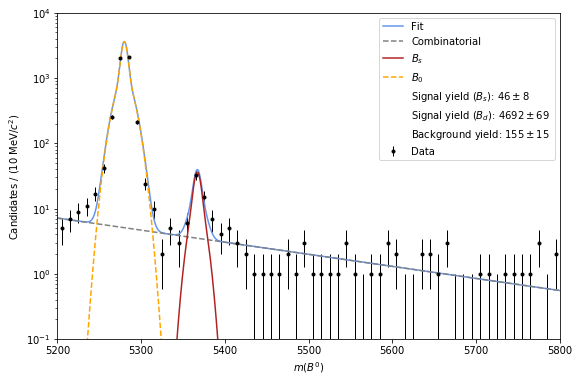
\includegraphics[width=0.7\linewidth]{plots/data_fit.png}
	\caption{Fit to the invariant mass spectrum of the BDT selected data, consisting of a signal, control and background component.}
	\label{fig:fit}
\end{figure}
In total, $46\pm8$ $B_s$ candidates are observed. The significance of this peak is calculated as $S = 5.56 \, \sigma$ with the help of \eqref{eq:sig}.
The number of background and signal events is obtained by integrating the individual functions of the signal and background component over the signal intervall.
All of the parameters of these functions are obtained in the previous fit.